% Finding the grid, reading the digits, solving (slides 4-10). Presented by Leonardo.

% 4
\begin{frame}{Finding the grid}
  \withpic{\pic{grid_threshold.jpg}\hspace{1em}\pic{grid_contour.jpg}}{An adaptive threshold turns
  the ink white and the paper black. The grid is the largest contour with four corners.}
\end{frame}

% 5
\begin{frame}{Flattening the grid}
  \withpic{\pic{grid_contour.jpg}\hspace{1em}\pic{grid_lines.jpg}}{The four corners give a
  homography, which flattens the grid into a square. It is a Sudoku only if there is a line at every
  cell border.}
\end{frame}

% 6
\begin{frame}{Objects touching the grid}
  \withpic{\pic{merged_contour.jpg}\hspace{1em}\pic{merged_refined.jpg}}{When an object touches the
  grid, the contour goes around both. We start from the four corners of its convex hull, and move each
  corner a little at a time while the cell borders line up better.}
\end{frame}

% 7
\begin{frame}{Printed digits}
  \withpic{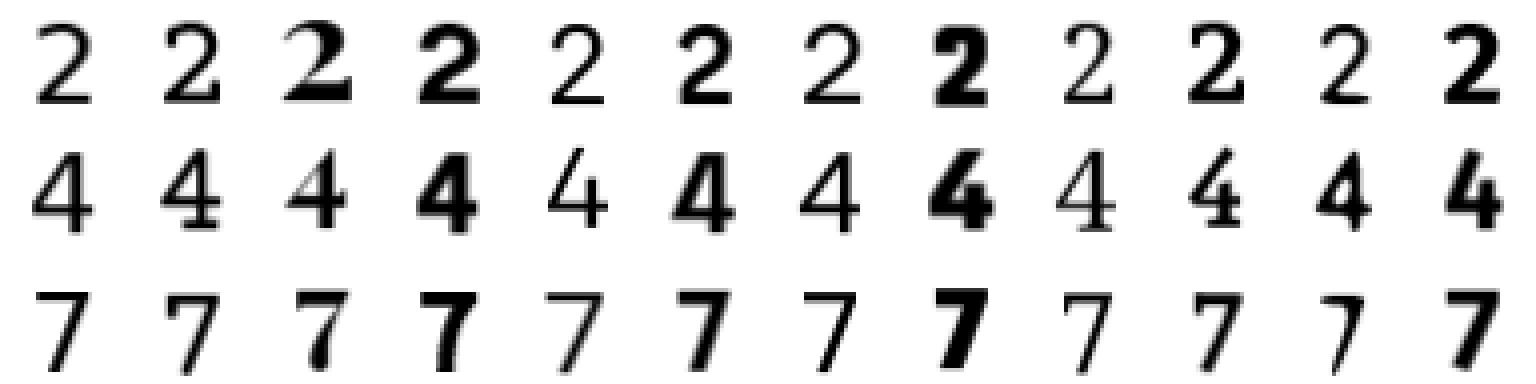
\includegraphics[width=0.6\textwidth]{figures/templates.png}}{Each digit is compared
  with the digits 1 to 9 in many fonts, and the best match gives the digit. We try the grid in four
  rotations: the one that matches best is the right way up.}
\end{frame}

% 8
\begin{frame}{Printed or handwritten}
  \withpic{\pic[0.4\textheight]{digits_flat.jpg}\hspace{1em}\pic[0.4\textheight]{digits_read.jpg}}%
  {A digit is printed if it matches a font well and is as dark and as tall as the other printed
  ones. Handwritten digits are described with HOG, a histogram of edge directions, and get the label
  of the closest MNIST digits.}
\end{frame}

% 9
\begin{frame}{Solving}
  \withpic{\pic{mistakes.jpg}}{Backtracking solves the puzzle from the printed digits. A
  proper Sudoku has only one solution, so a handwritten digit that differs from it is a mistake.}
\end{frame}

% 10
\begin{frame}{The order of the digits}
  \withpic{\pic{order.jpg}}{We show the digits in the order a person would find them, starting from
  the cells where only one digit fits.}
\end{frame}
